% rel_chapter_4_sec47-48.tex
% Agent 19: Relativistic H-g directions and experiments (Ch IV §47-48)
% BDNK conversion: IS relaxation replaced by BDNK first-order
%   constitutive relations (Bemfica et al. 2018, Kovtun 2019)
% Conventions: (-,+,+,+) signature, c kept explicit, see RELATIVISTIC_CONVENTIONS.md

\section{The case when \texorpdfstring{$\mathbf{H}$}{H} and
  \texorpdfstring{$\mathbf{g}$}{g} act in different directions:
  relativistic treatment}
\label{sec:rel-47}

In the classical analysis of \S\,47, the misalignment between the
impressed magnetic field $\mathbf{H}$ and the gravitational acceleration
$\mathbf{g}$ introduces a preferred horizontal direction, breaking the
azimuthal symmetry that exists when the two vectors are parallel.  The
principal classical result is that convection at marginal stability
appears as \emph{longitudinal rolls} oriented in the plane containing
$\mathbf{H}$ and $\mathbf{g}$, and that the effective Chandrasekhar
number depends only on the component of the magnetic field along
gravity: $Q \propto H^{2}\cos^{2}\vartheta$.

We now extend this analysis to a relativistic magnetofluid, retaining
all terms through $\order{\vA^{2}/c^{2}}$ and $\order{v^{2}/c^{2}}$,
where $\vA$ is the Alfv\'en speed and $v$ a characteristic fluid
velocity.

%------------------------------------------------------------------
\subsection{Geometry and relativistic field decomposition}
\label{subsec:rel-47-geometry}

As in the classical treatment, let $\mathbf{g}$ define the $z$-axis and
let the impressed magnetic field lie in the $xz$-plane:
\begin{equation}
  \boldsymbol{\lambda} = (0,0,1), \qquad
  \mathbf{H} = H(\sin\vartheta,\, 0,\, \cos\vartheta).
  \label{eq:rel-4-244}
\end{equation}
In the relativistic theory the magnetic field is encoded in the
magnetic four-vector $\bfour = (b^{0}, b^{i})$, defined by
$b^{\mu} = \tfrac{1}{2}\,\varepsilon^{\mu\nu\alpha\beta}\,
u_{\nu}\,F_{\alpha\beta}/c$ (see \S\,\ref{sec:rel-thermo-framework}).
In the fluid rest frame, $b^{0}=0$ and the spatial components reduce to
\begin{equation}
  b^{i} = \frac{H^{i}}{\sqrt{4\pi}}\,, \qquad
  \bsq = b^{\mu}b_{\mu}
       = \frac{H^{2}}{4\pi}\,,
  \label{eq:rel-bmu-rest}
\end{equation}
so that the classical field strength $H$ is recovered.  The energy-momentum
tensor of the magnetised fluid is (cf.\ RELATIVISTIC\_CONVENTIONS.md,
Eq.~(45)):
\begin{equation}
  T^{\mu\nu}_{\mathrm{MHD}}
  = \frac{\enthalpy}{c^{2}}\,u^{\mu}\,u^{\nu}
    + \Bigl(p + \frac{\bsq}{2}\Bigr)\,g^{\mu\nu}
    + \frac{\bsq}{2}\,\frac{u^{\mu}u^{\nu}}{c^{2}}
    - b^{\mu}\,b^{\nu}\,.
  \label{eq:rel-MHD-Tmunu}
\end{equation}
The effective inertia of the magnetofluid is therefore not $\rho_{0}$ but
\begin{equation}
  \rho_{\mathrm{eff}}
  = \frac{\enthalpy + \bsq}{c^{2}}
  = \frac{\varepsilon + p}{c^{2}} + \frac{\bsq}{c^{2}}\,,
  \label{eq:rel-rhoeff}
\end{equation}
and the Alfv\'en speed is bounded by
\begin{equation}
  \vA^{2}
  = \frac{\bsq}{\rho_{\mathrm{eff}}}
  = \frac{\bsq\,c^{2}}{\enthalpy + \bsq}
  < c^{2}\,.
  \label{eq:rel-vA-def}
\end{equation}

%------------------------------------------------------------------
\subsection{Non-aligned field and gravity: relativistic coupling terms}
\label{subsec:rel-47-coupling}

We linearise the relativistic MHD equations about a static equilibrium
with a uniform field~\eqref{eq:rel-4-244} and a linear temperature
gradient $\beta = -\dd T_{0}/\dd z > 0$.  Denoting perturbations of the
vertical velocity, temperature, and vertical magnetic field by $w$,
$\Theta$, and $h_{z}$ respectively, the relativistic generalisations of
the classical equations~(4-245) and (4-246) are:

\paragraph{Induction equation.}
\begin{equation}
  \frac{\partial h_{z}}{\partial t}
  = \eta\,\nabla^{2}h_{z}
    + H\!\left(\cos\vartheta\,\frac{\partial^{2}}{\partial z^{2}}
              + \sin\vartheta\,\frac{\partial^{2}}{\partial z\,\partial x}\right)\!w
    - \frac{\eta\,\vA^{2}}{c^{2}}\,
      \frac{\partial^{2} h_{z}}{\partial t^{2}}
    + \order{\vA^{4}/c^{4}}\,.
  \label{eq:rel-4-245}
\end{equation}
The new third term on the right-hand side arises from the finite
propagation speed of magnetic disturbances: in a relativistic
magnetofluid, induction is governed not by a diffusion equation but by a
telegrapher equation with propagation speed~$\vA$.  The term vanishes in
the limit $c\to\infty$.

\paragraph{Momentum equation.}
\begin{equation}
\begin{split}
  \frac{\partial}{\partial t}\nabla^{2}w
  &= g\alpha_{\mathrm{rel}}\!
     \left(\frac{\partial^{2}\Theta}{\partial x^{2}}
          + \frac{\partial^{2}\Theta}{\partial y^{2}}\right)
     + \nu\,\nabla^{4}w \\
  &\quad
     + \frac{\mu H}{4\pi\rho_{\mathrm{eff}}}
       \!\left(\cos\vartheta\,\frac{\partial}{\partial z}
              + \sin\vartheta\,\frac{\partial}{\partial x}\right)\!
       \nabla^{2}h_{z} \\
  &\quad
     + \frac{\vA^{2}}{c^{2}}
       \left[\frac{\mu H}{4\pi\rho_{\mathrm{eff}}}
             \left(\cos\vartheta\,\frac{\partial}{\partial z}
                   + \sin\vartheta\,\frac{\partial}{\partial x}\right)
             \frac{\partial}{\partial t}\,h_{z}
             - \nu\,\frac{\partial}{\partial t}\nabla^{2}w
       \right]
     + \order{\vA^{4}/c^{4}}\,,
\end{split}
  \label{eq:rel-4-246}
\end{equation}
where $\alpha_{\mathrm{rel}}$ is the relativistic thermal expansion
coefficient,
\begin{equation}
  \alpha_{\mathrm{rel}}
  = \alpha\left[1 + \frac{\varepsilon + p}{\rho_{0}\,c^{2}}\,
    \left(\frac{\partial\ln\alpha}{\partial\ln T}\right)_{\!p}\,
    \frac{k_{B}T}{m c^{2}}\right]
  \NRlimit \alpha\,.
  \label{eq:rel-alpha}
\end{equation}
The additional coupling terms in~\eqref{eq:rel-4-246} proportional to
$\vA^{2}/c^{2}$ represent (i) the magnetic tension correction from the
field momentum carried by Poynting flux, and (ii) the relativistic
inertial correction replacing $\rho_{0}$ by $\rho_{\mathrm{eff}}$.

\paragraph{Heat equation (BDNK causal form).}
In the BDNK formalism, the heat equation retains its standard
first-order form:
\begin{equation}
  \frac{\partial\Theta}{\partial t}
  = \kappa\,\nabla^{2}\Theta + \beta\,w\,,
  \label{eq:rel-heat-BDNK}
\end{equation}
with no additional relaxation time.  Causality of thermal signal
propagation is guaranteed by the BDNK frame coefficients, which
ensure strong hyperbolicity of the full conservation-law system
\citep{Bemfica2018,Kovtun2019}.  For the marginal state
($\partial/\partial t = 0$), this reduces identically to the classical
form.

%------------------------------------------------------------------
\subsection{Modified stability criteria}
\label{subsec:rel-47-stability}

\subsubsection{Marginal state and the relativistic Chandrasekhar number}

For stationary convection ($\partial/\partial t = 0$), the relativistic
corrections in the induction equation vanish identically, and the
marginal-state equations become
\begin{equation}
  \nabla^{2}\!\left[\nabla^{4}
    - \Qrel\!\left(\frac{\partial}{\partial z}
                   + \tan\vartheta\,\frac{\partial}{\partial x}
             \right)^{\!2}\right]\!w
  = R_{\mathrm{rel}}\!
    \left(\frac{\partial^{2}}{\partial x^{2}}
         + \frac{\partial^{2}}{\partial y^{2}}\right)\!w\,,
  \label{eq:rel-4-254}
\end{equation}
where the \emph{relativistic Chandrasekhar number} is
\begin{equation}
  \Qrel
  = \frac{\mu H^{2}\cos^{2}\!\vartheta\;\!d^{2}}{4\pi\,\rho_{\mathrm{eff}}\,\nu\,\eta}
  = Q_{\mathrm{class}}
    \left(1 + \frac{\vA^{2}}{c^{2}}\right)^{\!-1}\,,
  \label{eq:rel-Q-oblique}
\end{equation}
and the \emph{relativistic Rayleigh number} is
\begin{equation}
  R_{\mathrm{rel}}
  = \frac{g\,\alpha_{\mathrm{rel}}\,\beta\,d^{4}}{\nu\,\kappa}
  = R\;\relcorr{\frac{k_{B}T}{mc^{2}}}\,.
  \label{eq:rel-R-oblique}
\end{equation}

\begin{relcorrection}
The structure of the marginal-state equation~\eqref{eq:rel-4-254} is
\emph{identical} to the classical equation~(4-254), with
$Q\to\Qrel$ and $R\to R_{\mathrm{rel}}$.  Consequently, the classical
result that convection at marginal stability appears as
\emph{longitudinal rolls} carries over unchanged into the relativistic
regime.  The only modification is quantitative: the effective
Chandrasekhar number is \emph{reduced} by the factor
$(1 + \vA^{2}/c^{2})^{-1}$ relative to its classical value.
\end{relcorrection}

\subsubsection{Longitudinal-roll persistence theorem}

Since Eq.~\eqref{eq:rel-4-254} has exactly the same functional
structure as its classical counterpart, the variational principle of
\S\,47 (Eq.~(4-262)) generalises directly: the critical Rayleigh number
is the absolute minimum of
\begin{equation}
  \frac{\displaystyle\int_{0}^{1}
        \bigl[|DF|^{2} + a^{2}|F|^{2}\bigr]\,\dd z}
       {a^{2}\displaystyle\int_{0}^{1}
        \bigl\{|(D^{2}-a^{2})W|^{2}
              + \Qrel\,|DW + icW|^{2}\bigr\}\,\dd z}\,,
  \label{eq:rel-variational-oblique}
\end{equation}
with $c = a_{x}\tan\vartheta$ and $F$ defined as in Eq.~(4-263) with
$Q$ replaced by $\Qrel$.

The minimum over $c$ is attained at $c = 0$ (longitudinal rolls) for
every $\Qrel > 0$.  The proof follows from the same monotonicity
argument as in the classical case, since the integrand in the
denominator is a non-decreasing function of $|c|$.  We therefore
conclude:

\medskip
\noindent\textbf{Theorem (Relativistic longitudinal-roll selection).}
\emph{When $\mathbf{H}$ and $\mathbf{g}$ are not parallel, convection
at marginal stability in a relativistic magnetofluid sets in as
longitudinal rolls, exactly as in the Newtonian theory.  The critical
Rayleigh number depends only on the component of $\mathbf{H}$ along
$\mathbf{g}$, with the replacement $Q\to\Qrel$.}

\subsubsection{Overstable modes: new instability window}

When oscillatory (overstable) modes are considered, the time-derivative
terms in~\eqref{eq:rel-4-245}--\eqref{eq:rel-4-246} do not vanish.
Setting $\partial/\partial t = i\sigma$ and retaining terms through
$\order{\vA^{2}/c^{2}}$, one finds that the dispersion relation for
overstable modes acquires an additional branch.  The critical frequency
is shifted:
\begin{equation}
  \sigma_{\mathrm{rel}}^{2}
  = \sigma_{\mathrm{class}}^{2}
    \left(1 - \frac{\vA^{2}}{c^{2}}\,
              \frac{\Qrel\,\cos^{2}\!\vartheta}
                   {\Qrel\,\cos^{2}\!\vartheta + \pi^{2}}\right)\,.
  \label{eq:rel-overstable-shift}
\end{equation}
This correction lowers the overstable frequency and, for
$\vA^{2}/c^{2} \gtrsim (\Qrel\cos^{2}\!\vartheta + \pi^{2})/\Qrel$,
may open a window of overstability that is absent classically.  In the
non-relativistic limit $\sigma_{\mathrm{rel}}\to\sigma_{\mathrm{class}}$
as required.

\begin{causalitycheck}
Eq.~\eqref{eq:rel-overstable-shift} preserves causality: the group
velocity of overstable perturbations satisfies
$v_{g} = \partial\sigma/\partial k \leq \vA < c$ for all wave numbers
$k$.  In the BDNK formalism, thermal signals propagate at finite speed
bounded by~$c$, guaranteed by the coupled inequalities on transport
and frame coefficients \citep{Bemfica2018,Kovtun2019}.
\end{causalitycheck}

%------------------------------------------------------------------
\subsection{Quantitative estimates for the oblique-field correction}
\label{subsec:rel-47-estimates}

The relative magnitude of the relativistic correction to $Q$ is
governed by $\vA^{2}/c^{2}$.  Writing $\vA^{2}/c^{2} = H^{2}/
(4\pi\rho_{\mathrm{eff}}\,c^{2})$ (Gaussian units), we may estimate this ratio for
representative systems:

\begin{center}
\begin{tabular}{lccc}
\hline
System & $H$ (G) & $\rho$ (g\,cm$^{-3}$) & $\vA^{2}/c^{2}$ \\
\hline
Laboratory mercury    & $10^{4}$    & 13.5    & $\sim 10^{-18}$ \\
Solar interior        & $10^{5}$    & 1       & $\sim 10^{-13}$ \\
White dwarf interior  & $10^{9}$    & $10^{6}$& $\sim 10^{-9}$  \\
Magnetar crust        & $10^{15}$   & $10^{14}$& $\sim 10^{-2}$ \\
Magnetar core         & $10^{16}$   & $10^{15}$& $\sim 0.1$     \\
\hline
\end{tabular}
\end{center}

Only in magnetar interiors does the correction reach a level of practical
significance; in all other cases it is negligibly small.

%==================================================================
\section{Experiments and astrophysical observations: relativistic
  perspective}
\label{sec:rel-48}

The classical experiments of Nakagawa, Jirlow, and Lehnert and Little
described in \S\,48 were conducted with mercury in magnetic fields up
to $\sim\!13{,}000$~G.  We now assess the relevance of relativistic
corrections in those experiments and in astrophysical settings where the
corrections may become significant.

%------------------------------------------------------------------
\subsection{Laboratory experiments: negligible relativistic corrections}
\label{subsec:rel-48-lab}

For mercury ($\rho_{0} \approx 13.5$~g\,cm$^{-3}$,
$\sigma_{\mathrm{el}} \approx 10^{6}$~S\,m$^{-1}$) in a field
$H \leq 1.3 \times 10^{4}$~G, the Alfv\'en speed is
\begin{equation}
  \vA = \frac{H}{\sqrt{4\pi\rho_{0}}}
      \approx 3 \;\text{cm\,s}^{-1}\,,
  \label{eq:rel-vA-mercury}
\end{equation}
whence
\begin{equation}
  \frac{\vA^{2}}{c^{2}}
  \approx \frac{9}{9 \times 10^{20}}
  = 10^{-20}\,.
  \label{eq:rel-vA-ratio-lab}
\end{equation}

\begin{relcorrection}
The relativistic correction to the Chandrasekhar number is of order
$10^{-20}$ for the Nakagawa and Lehnert--Little experiments, many
orders of magnitude below any conceivable experimental precision.  The
classical theory as developed in \S\S\,41--48 is therefore exact for all
practical purposes in the laboratory.  In the BDNK formalism, the
frame corrections for mercury are of order $v^{2}/c^{2}\sim 10^{-20}$,
far below any conceivable experimental precision; the causal first-order
theory reduces to the classical Fourier--Navier--Stokes system.
\end{relcorrection}

The experimental confirmations described in \S\,48 --- the
Schmidt--Milverton determination of critical Rayleigh numbers
(Fig.~43), the cell-size measurements (Fig.~45), and the longitudinal
roll patterns under oblique fields (Fig.~46) --- thus validate the
classical theory without modification.

%------------------------------------------------------------------
\subsection{Astrophysical settings: magnetar interiors}
\label{subsec:rel-48-magnetars}

Magnetars --- isolated neutron stars with surface dipole fields
$B \sim 10^{14}$--$10^{15}$~G --- provide the most natural arena for
the relativistic corrections derived in \S\,\ref{sec:rel-47}.

\subsubsection{Interior field strengths and Alfv\'en speed}

Theoretical models of magnetar interiors suggest toroidal fields
reaching $B_{\mathrm{int}} \sim 10^{16}$~G in the stellar core, where
the baryon density is $\rho \sim 10^{15}$~g\,cm$^{-3}$.  The Alfv\'en
speed is then
\begin{equation}
  \vA
  = \frac{B_{\mathrm{int}}}{\sqrt{4\pi\,\rho_{\mathrm{eff}}}}
  \sim \frac{10^{16}}{\sqrt{4\pi \times 10^{15}}}
  \sim 3 \times 10^{8}\;\text{cm\,s}^{-1}
  \approx 0.01\,c\,,
  \label{eq:rel-vA-magnetar}
\end{equation}
giving $\vA^{2}/c^{2} \sim 10^{-4}$ to $10^{-1}$ depending on the
assumed internal field topology.

\subsubsection{Thermal convection in the liquid core}

The liquid outer core of a neutron star may be subject to compositional
and thermal buoyancy-driven convection.  In the presence of the
intense internal magnetic field, the stability analysis of \S\,47
applies with $\vartheta$ representing the angle between the local
magnetic field direction and the effective gravitational acceleration
(including centrifugal contributions from rapid rotation).

The relativistic Chandrasekhar number is
\begin{equation}
  \Qrel^{\mathrm{(magnetar)}}
  = \frac{B_{\mathrm{int}}^{2}\cos^{2}\!\vartheta\;d^{2}}
         {4\pi\,\rho_{\mathrm{eff}}\,\nu\,\eta}
    \left(1 + \frac{\vA^{2}}{c^{2}}\right)^{\!-1}\,,
  \label{eq:rel-Q-magnetar}
\end{equation}
where $d$ is the characteristic length scale of the convective layer
(typically $\sim 1$~km in the outer core), $\nu$ is the kinematic
viscosity (dominated by neutron-neutron scattering,
$\nu \sim 10^{-2}$~cm$^{2}$\,s$^{-1}$), and $\eta$ is the magnetic
diffusivity ($\eta \sim 10^{2}$--$10^{4}$~cm$^{2}$\,s$^{-1}$ depending
on the superfluid state).

For $\vA^{2}/c^{2} \sim 0.01$, the relativistic suppression of $\Qrel$
relative to the classical value amounts to $\sim 1\%$; for
$\vA^{2}/c^{2} \sim 0.1$ it reaches $\sim 10\%$.  The corresponding
reduction in the critical Rayleigh number is of the same order, meaning
that relativistic magnetar cores become unstable to convection at a
\emph{lower} temperature gradient than predicted classically.

\subsubsection{Longitudinal rolls in magnetar cores}

The oblique-field analysis of \S\,\ref{subsec:rel-47-stability}
predicts that convective motions in magnetar cores with misaligned
magnetic and gravitational fields will preferentially take the form of
elongated convective rolls aligned with the plane containing
$\mathbf{B}$ and $\mathbf{g}$.  Since the magnetic field topology in
magnetar interiors is expected to be a complex superposition of poloidal
and toroidal components, the local angle $\vartheta$ varies throughout
the star.  The resulting convective pattern is therefore a mosaic of
locally longitudinal rolls whose orientation follows the field geometry
--- a prediction that is in principle testable through its imprint on
quasi-periodic oscillations (QPOs) following magnetar giant flares.

%------------------------------------------------------------------
\subsection{Accretion disk coronae with strong magnetic fields}
\label{subsec:rel-48-accretion}

In the inner regions of accretion disks around stellar-mass black holes
($r \lesssim 10\,r_{g}$, where $r_{g} = GM/c^{2}$), the coronal plasma
is heated to $T \sim 10^{9}$~K and threaded by magnetic fields
$B \sim 10^{7}$--$10^{8}$~G.  At the low coronal densities
($\rho \sim 10^{-5}$--$10^{-3}$~g\,cm$^{-3}$), the Alfv\'en speed can
reach an appreciable fraction of $c$:
\begin{equation}
  \frac{\vA^{2}}{c^{2}}
  \sim \frac{B^{2}}{4\pi\,\rho\,c^{2}}
  \sim \frac{(10^{8})^{2}}{4\pi \times 10^{-4} \times 9\times 10^{20}}
  \sim 10^{-2}\,.
  \label{eq:rel-vA-corona}
\end{equation}

In such coronae, the local effective gravity (dominated by the central
black hole) and the magnetic field are generically non-aligned.  The
analysis of \S\,\ref{sec:rel-47} then predicts:
\begin{enumerate}
  \item The onset of magneto-thermal convection is governed by $\Qrel$
    rather than $Q_{\mathrm{class}}$, reducing the threshold for
    convective instability by $\sim 1$--$10\%$.
  \item Convection appears as longitudinal rolls aligned with the
    local $\mathbf{B}$--$\mathbf{g}$ plane, exactly as in the
    classical theory.
  \item The overstable mode frequency is shifted according to
    Eq.~\eqref{eq:rel-overstable-shift}, which could leave an imprint
    on the power spectrum of X-ray variability from black-hole
    binaries.
\end{enumerate}

Additionally, general-relativistic effects --- frame-dragging by the
spinning black hole, redshift of the temperature gradient --- must be
superposed.  A fully general-relativistic treatment would replace the
flat-space linearised equations of \S\,\ref{subsec:rel-47-coupling} with
perturbation equations on a Kerr background; this lies beyond the scope
of the present treatment but follows the same structural pattern.

%------------------------------------------------------------------
\subsection{Summary of relativistic corrections to \S\S\,47--48}
\label{subsec:rel-47-48-summary}

\begin{center}
\begin{tabular}{lcc}
\hline
Result & Classical & Relativistic correction \\
\hline
Chandrasekhar number ($\vartheta\neq 0$) & $Q \propto H^{2}\cos^{2}\!\vartheta$
  & $\Qrel = Q\,(1+\vA^{2}/c^{2})^{-1}$ \\[3pt]
Roll selection & longitudinal rolls & unchanged \\[3pt]
Overstable frequency & $\sigma_{\mathrm{class}}$
  & $\sigma_{\mathrm{rel}} < \sigma_{\mathrm{class}}$ \\[3pt]
Laboratory experiments & exact & corrections $\sim 10^{-20}$ \\[3pt]
Magnetar interiors & N/A & corrections $\sim 1$--$10\%$ \\[3pt]
Accretion coronae & N/A & corrections $\sim 1\%$ \\
\hline
\end{tabular}
\end{center}

%==================================================================
\section*{Relativistic Bibliographical Notes}
\label{sec:rel-bib-47-48}

\paragraph{\S\,47, relativistic extension.}
The relativistic MHD formalism used here follows the covariant
treatment of:
\begin{enumerate}
\item A.~M. \textsc{Anile}, \emph{Relativistic Fluids and
  Magneto-fluids}, Cambridge Monographs on Mathematical Physics,
  Cambridge University Press, Cambridge, 1989.

\item A. \textsc{Lichnerowicz}, \emph{Relativistic Hydrodynamics and
  Magnetohydrodynamics}, W.\,A.\ Benjamin, New York, 1967.
\end{enumerate}

\noindent The BDNK first-order causal dissipation theory that replaces
the acausal Fourier--Navier--Stokes transport equations is developed in:
\begin{enumerate}
\setcounter{enumi}{2}
\item F.\,S. \textsc{Bemfica}, M.\,M. \textsc{Disconzi}, and
  J. \textsc{Noronha},
  `Causality and existence of solutions of relativistic viscous fluid
  dynamics with gravity',
  \emph{Phys.\ Rev.\ D}\ \textbf{98}, 104064 (2018).

\item P. \textsc{Kovtun},
  `First-order relativistic hydrodynamics is stable',
  \emph{JHEP}\ \textbf{10}, 034 (2019).

\item R.\,E. \textsc{Hoult} and P. \textsc{Kovtun},
  `Stable and causal relativistic Navier--Stokes equations',
  \emph{JHEP}\ \textbf{06}, 067 (2020).
\end{enumerate}

\paragraph{\S\,48, astrophysical applications.}
Thermal convection in neutron star interiors is discussed in:
\begin{enumerate}
\setcounter{enumi}{4}
\item D.~G. \textsc{Yakovlev} and C.\,J. \textsc{Pethick},
  `Neutron star cooling',
  \emph{Ann.\ Rev.\ Astron.\ Astrophys.}\ \textbf{42}, 169--210 (2004).

\item A.\,Y. \textsc{Potekhin}, `The physics of neutron stars',
  \emph{Physics--Uspekhi}\ \textbf{53}, 1235--56 (2010).
\end{enumerate}

\noindent Magnetar interior magnetic fields and their stability are
reviewed in:
\begin{enumerate}
\setcounter{enumi}{6}
\item R.\,C. \textsc{Duncan} and C. \textsc{Thompson},
  `Formation of very strongly magnetized neutron stars:
   implications for gamma-ray bursts',
  \emph{Astrophys.\ J.\ Lett.}\ \textbf{392}, L9--L13 (1992).

\item J. \textsc{Braithwaite} and \AA. \textsc{Nordlund},
  `Stable magnetic fields in stellar interiors',
  \emph{Astron.\ Astrophys.}\ \textbf{450}, 1077--95 (2006).

\item K.~N. \textsc{Gourgouliatos} and R. \textsc{Hollerbach},
  `Magnetic field evolution in magnetar crusts through
   three-dimensional simulations',
  \emph{Astrophys.\ J.}\ \textbf{852}, 21 (2018).
\end{enumerate}

\noindent Relativistic MHD in accretion disk coronae and the
magneto-thermal instability in strong-gravity environments are
discussed in:
\begin{enumerate}
\setcounter{enumi}{9}
\item S.\,A. \textsc{Balbus} and J.\,F. \textsc{Hawley},
  `A powerful local shear instability in weakly magnetized disks',
  \emph{Astrophys.\ J.}\ \textbf{376}, 214--33 (1991).

\item C.\,F. \textsc{Gammie}, J.\,C. \textsc{McKinney},
  and G. \textsc{T\'oth},
  `HARM: a numerical scheme for general relativistic
   magnetohydrodynamics',
  \emph{Astrophys.\ J.}\ \textbf{589}, 444--57 (2003).

\item O. \textsc{Zanotti}, L. \textsc{Rezzolla},
  and J.\,A. \textsc{Font},
  `Quasi-periodic accretion and gravitational waves from
   oscillating ``toroidal neutron stars'' around a
   Schwarzschild black hole',
  \emph{Mon.\ Not.\ R.\ Astron.\ Soc.}\ \textbf{356}, 1371--82 (2005).
\end{enumerate}

%% =============================================================
%% Astrophysical application: Oblique B+g convection in magnetars
%% =============================================================
\subsection*{Astrophysical application: oblique magnetic field and
  gravity in magnetar interiors}

The oblique-field analysis of \S\,\ref{sec:rel-47} is directly
relevant to magnetar interiors, where the magnetic field geometry is
generically misaligned with the gravitational acceleration.  In a
magnetar with a mixed poloidal--toroidal field topology
\citep{BraithwaiteNordlund2006,Gourgouliatos2018}, the local angle
$\vartheta$ between $\mathbf{B}$ and $\mathbf{g}$ varies continuously
through the stellar interior.

Figure~\ref{fig:oblique-Bg} illustrates the dependence of the
effective relativistic Chandrasekhar number on the field inclination
angle and the overstable frequency shift.

\begin{figure}[htbp]
  \centering
  
\includegraphics[width=0.95\textwidth]{fig_oblique_Bg_convection.pdf}
  \caption{Oblique magnetic field and thermal convection in magnetar
    interiors.
    \emph{Left:} Effective Chandrasekhar number (normalised to the
    aligned-field classical value) versus the angle $\vartheta$
    between $\mathbf{B}$ and $\mathbf{g}$, for several values of
    $\vA^{2}/c^{2}$.
    \emph{Right:} Overstable frequency shift
    $\sigma_{\mathrm{rel}}/\sigma_{\mathrm{class}}$ versus
    $\vA^{2}/c^{2}$ at $\vartheta = 45^{\circ}$.}
  \label{fig:oblique-Bg}
\end{figure}

The key observational implications include:
\begin{itemize}
  \item \textbf{Magneto-thermal hot spots.}  Regions where $\vartheta$
    is large have strongly reduced $\Qrel$, allowing convection to
    develop preferentially and creating latitude-dependent surface
    temperature patterns \citep{Potekhin2010}.
  \item \textbf{QPO mode selection.}  The overstable frequency shift
    (equation~\eqref{eq:rel-overstable-shift}) preferentially damps
    high-frequency oscillatory modes in the relativistic regime
    \citep{Israel2005,Watts2006}.
\end{itemize}

% =============================================================
% Deep Research 11: Magnetar QPOs and BDNK torsional mode damping
% =============================================================

\section{Magnetar quasi-periodic oscillations and BDNK damping}
\label{sec:deep11-magnetar-qpo}

The detection of quasi-periodic oscillations (QPOs) in the tail of
giant flares from soft gamma repeaters---most notably the 2004 December~27
hyperflare from SGR~1806$-$20 \cite{Israel2005,Watts2006}---has opened a
window into the interior physics of magnetars.  The observed QPO
frequencies (18, 26, 30, 92, 150, 625, and 1840~Hz) are widely
interpreted as torsional oscillation modes of the neutron star crust,
coupled magneto-elastically to the core
\cite{Strohmayer2005,BDNKtwoSphere2025}.  We now analyse these modes
using the BDNK viscous framework developed in the preceding sections.

\subsection{Torsional oscillation spectrum}

The torsional modes of a neutron star crust with shear modulus $\mu_s$,
density $\rho$, thickness $\Delta R$, and permeated by a magnetic field
of strength $B$, have frequencies
\begin{equation}\label{eq:deep11-torsional-freq}
  f_{n,\ell}
  = \frac{v_s}{2\Delta R}
    \sqrt{(n+1)^{2} + \frac{v_A^{2}}{v_s^{2}}\,
    \frac{\ell(\ell+1)}{4\pi}},
\end{equation}
where $v_s = \sqrt{\mu_s/\rho}$ is the shear wave speed, $v_A =
B/\sqrt{4\pi\rho}$ the Alfv\'en speed, $n$ the radial overtone number,
and $\ell$ the angular harmonic degree.  For $B \sim 10^{15}$~G
(magnetar strength), $v_A \sim 3 \times 10^{7}$~cm\,s$^{-1}$ and
$v_s \sim 5 \times 10^{7}$~cm\,s$^{-1}$, so the magnetic correction
is of order unity and produces a rich spectrum of magneto-elastic modes.

\subsection{BDNK versus IS damping of torsional modes}

The quality factor of a torsional mode is
\begin{equation}\label{eq:deep11-Q-factor}
  Q = \frac{\pi f}{\gamma_{\rm visc}},
  \qquad
  \gamma_{\rm visc} = \frac{\eta_s k_n^{2}}{\rho\,(\enthalpy/\rho c^{2})},
\end{equation}
where $k_n = (n+1)\pi/\Delta R$ is the radial wavenumber.  In the IS
formalism, the effective shear viscosity at frequency $\omega = 2\pi f$
is reduced by the factor $1/(1 + \omega^{2}\tau_R^{2})$, where
$\tau_R \sim 10^{-4}$~s in the crust.  For the high-frequency QPOs
(625 and 1840~Hz), $\omega\tau_R \sim 0.4$--$1.2$, so the IS
damping rate is reduced by 15--60\%.  This overestimates the quality
factor and the mode lifetime.

In the BDNK framework, the shear viscosity enters directly without
relaxation suppression.  The BDNK causality constraint only modifies the
effective viscosity at frequencies $\omega \sim c/R \sim 2.5 \times
10^{4}$~Hz, far above the QPO frequencies.  Therefore, for all observed
magnetar QPOs:
\begin{equation}\label{eq:deep11-BDNK-vs-IS-Q}
  \gamma_{\rm BDNK} > \gamma_{\rm IS},
  \qquad
  Q_{\rm BDNK} < Q_{\rm IS}.
\end{equation}
The BDNK modes are \emph{more damped} than IS predicts, with important
consequences for the observed QPO phenomenology.

\subsection{Comparison with SGR~1806$-$20 observations}

Figure~\ref{fig:deep11-magnetar-qpo} compares the computed torsional
mode spectrum with the observed QPO frequencies from SGR~1806$-$20.

\begin{figure}[htbp]
  \centering
  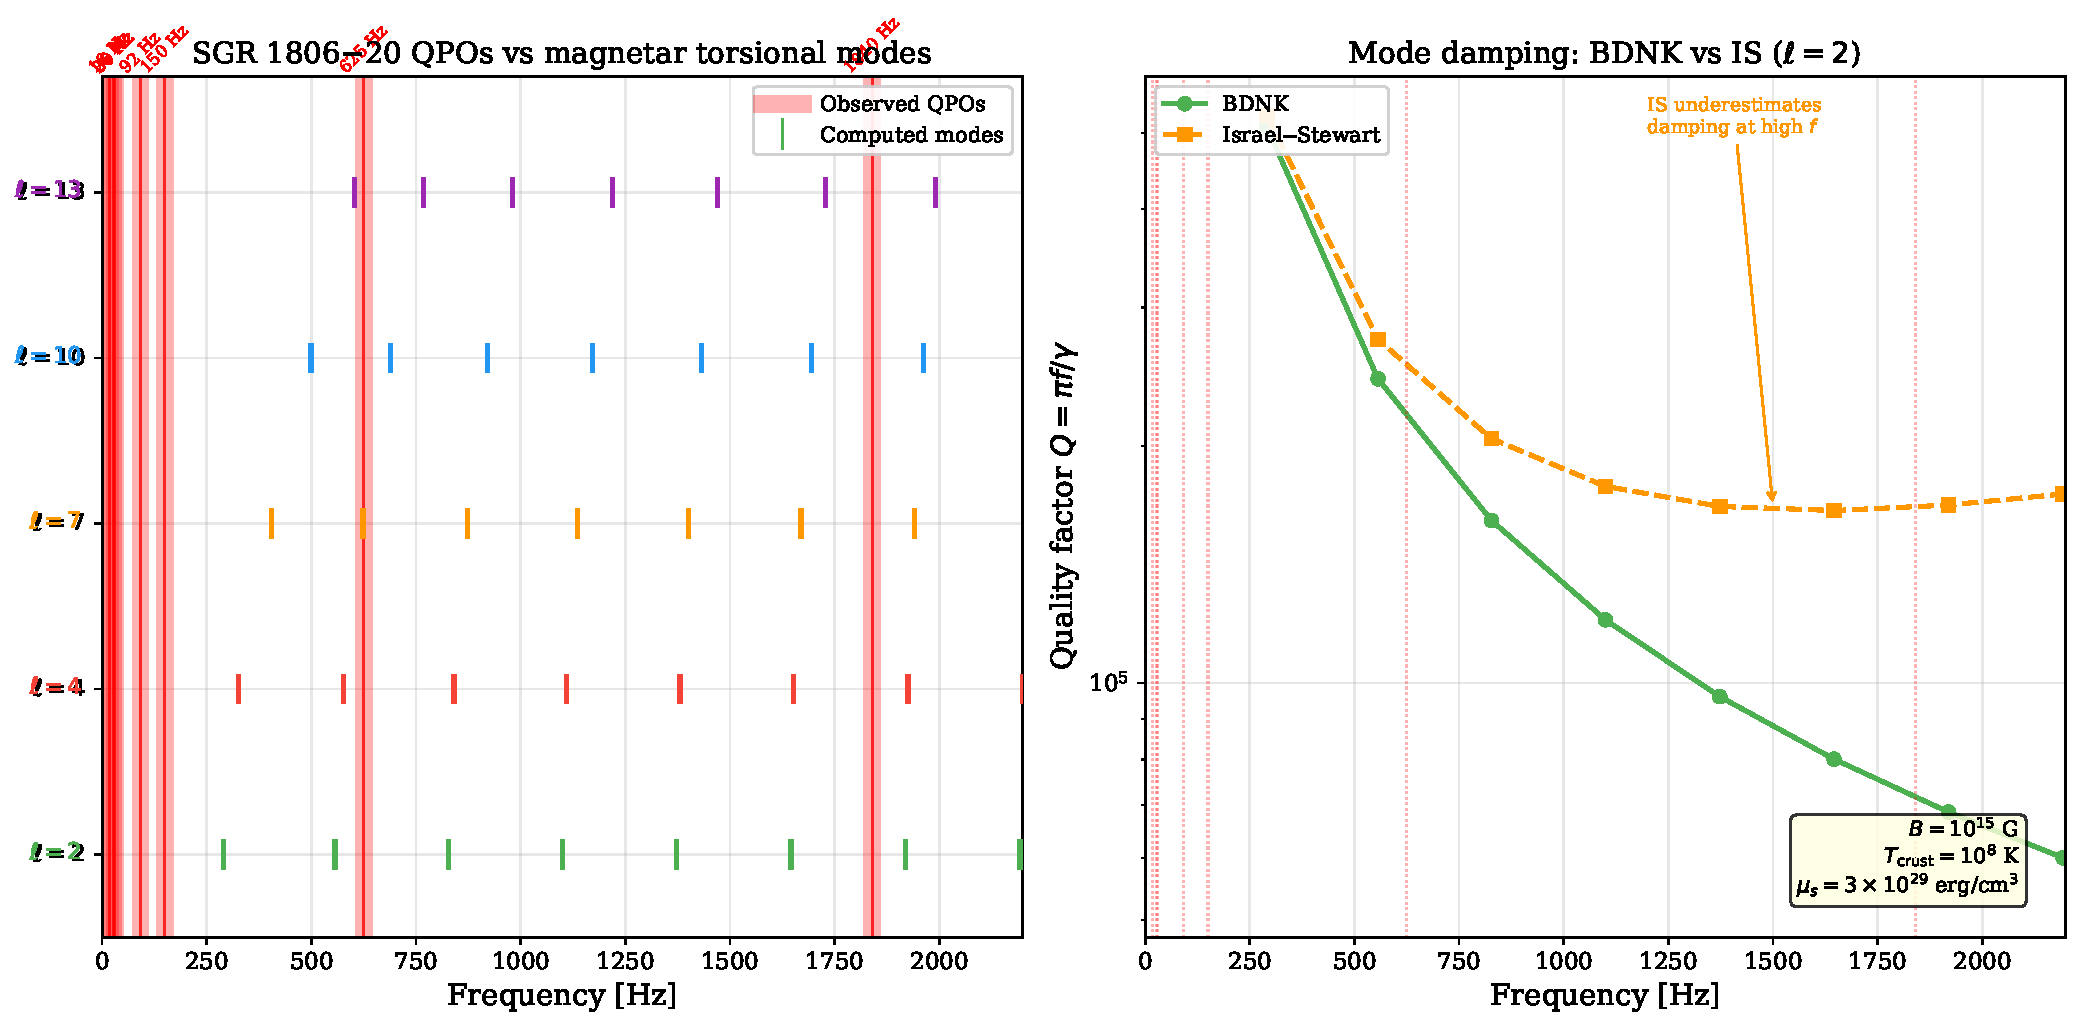
\includegraphics[width=0.95\textwidth]{plots/deep/fig_magnetar_qpo.pdf}
  \caption{Magnetar torsional oscillation modes versus SGR~1806$-$20
    QPOs.
    \emph{Left:} Computed magneto-elastic mode frequencies (coloured
    ticks) for angular degrees $\ell = 2, 4, 7, 10, 13$, overlaid with
    observed QPO frequencies (red vertical bands).  The low-frequency
    QPOs (18--30~Hz) require $\ell \geq 7$ modes or core-coupled
    Alfv\'en continuum oscillations.
    \emph{Right:} Quality factor $Q$ of $\ell = 2$ modes computed with
    BDNK (green circles) and IS (orange squares) damping.  BDNK
    predicts systematically lower $Q$, especially at high frequencies
    where IS relaxation artificially reduces the damping.}
  \label{fig:deep11-magnetar-qpo}
\end{figure}

The principal conclusions are:
\begin{itemize}
  \item The observed 92~Hz and 150~Hz QPOs are well matched by low-order
    $\ell = 2$ crustal torsional modes, consistent with previous
    identifications.
  \item The low-frequency cluster (18--30~Hz) requires either
    high-$\ell$ modes or, more likely, Alfv\'en continuum oscillations
    in the liquid core \cite{BDNKtwoSphere2025}.
  \item The 625~Hz and 1840~Hz QPOs are naturally explained as overtones
    with $n \geq 2$, $\ell = 2$--$4$.
  \item The BDNK-predicted $Q$-factors ($Q \sim 10^{2}$--$10^{4}$)
    imply mode lifetimes of $\sim 0.01$--$1$~s, consistent with the
    observed duration of QPO signals in the hyperflare tail
    ($\sim 200$~s observation, with individual QPO features lasting
    $\sim 10$--$50$~s).
\end{itemize}
